\section{Mon Modèle}

Mon approche consiste à appliquer la méthode de \textcite{seyb24from} et l'optimisation subséquente de \textcite{xu25practical} à l'intérieur d'un volume défini par la boîte englobante de la courbe B-spline. Pour ce faire, il suffit de définir une fonction de moyenne et de choisir un noyau de covariance afin de définir le processus de Gauss.

Dans notre approche, chaque cheveu est représenté par une courbe à 4 points de contrôle dont chaque point encode une position 3D et un rayon ; c'est le format utilisé par Mitsuba. Les modèles de cheveux utilisés comptent plus d'un million de cheveux individuels.

Pour représenter une courbe par une surface implicite définie par processus de Gauss, il faut être capable d'évaluer la fonction de moyenne en tout point du volume lors de l'échantillonnage le long du rayon. Pour les modèles 3D, la moyenne peut être encodée dans un volume 3D (OpenVDB) en enregistrant la valeur approximative pour chaque cellule. Cette approche n'est toutefois pas applicable aux cheveux, car les brins sont très fins et nécessiteraient des cellules infiniment petites, ce qui serait prohibitif en mémoire. Une autre approche, utilisée dans Tungsten, consiste à représenter la moyenne de façon procédurale en définissant explicitement une expression analytique, comme $ax + b$ pour un plan. Cette option n'est pas applicable aux cheveux en raison de leur forme complexe qui ne se réduit pas à un polynôme simple. Une troisième approche procédurale est l'utilisation d'une fonction de distance signée. Si l'on connaît une SDF pour la surface considérée, sa valeur peut servir de fonction de moyenne pour le processus de Gauss. Malheureusement, il n'existe pas de SDF analytique connue pour une courbe de Bézier ou une courbe B-spline cubique. Nous utiliserons donc une technique d'approximation de la courbe par union de capsules.

Considérons l'exemple 2D d'une courbe B-spline : en la segmentant à intervalles constants de $t$ et en reliant les points par des segments droits, on obtient une approximation polygonale qui devient de plus en plus fidèle à mesure que l'intervalle diminue. Chaque segment peut être enveloppé d'une capsule dont le rayon reproduit le rayon du cheveu. En prenant l'union des SDF de toutes les capsules, on obtient la distance minimale vers le cheveu, ce qui constitue une distance signée utilisable comme fonction de moyenne. Une valeur négative indique que le point se trouve à l'intérieur de la surface.

En 3D, la même approche s'applique. Chaque courbe est subdivisée en 16 segments, ce qui donne 17 points obtenus par évaluation de la courbe B-spline à pas constants de $t$. À partir de ces 17 points, on définit 16 capsules. On peut ensuite procéder à l'échantillonnage le long du rayon en appliquant le bruit parcimonieux convolutionnel sur chaque échantillon.

\begin{figure}[H]
    \centering
    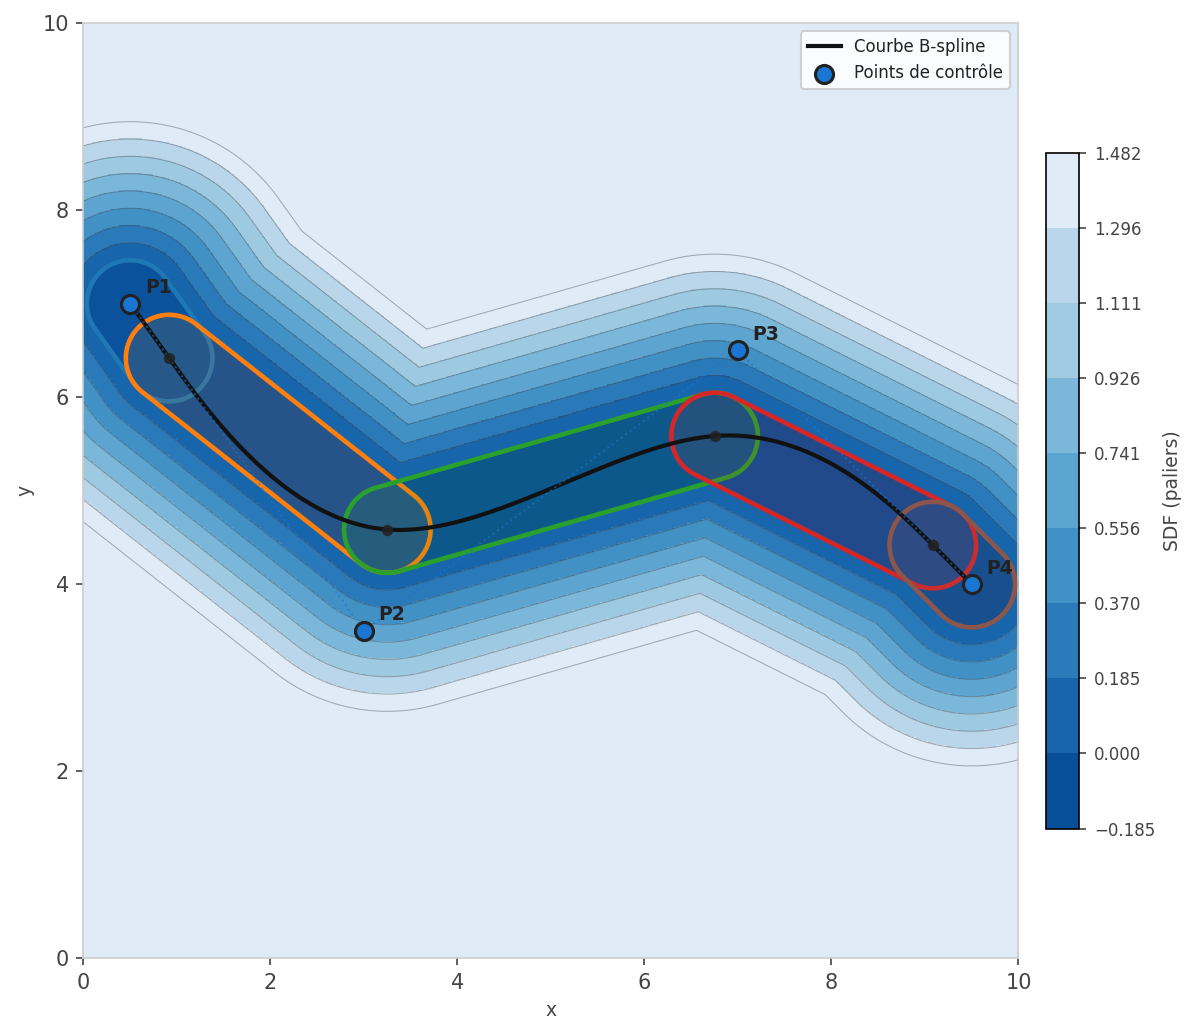
\includegraphics[width=0.8\textwidth]{figures/spline-sdf.png}
    \caption{Présentation visuelle du modèle : approximation d'une courbe B-spline par union de 5 capsules et évaluation de la SDF résultante.}
    \label{fig:spline_sdf}
\end{figure}

Pour le noyau de covariance, nous retenons le noyau squared exponential, car il garantit un rendu lisse, ce qui est souhaitable pour un cheveu individuel. Ce noyau sera approximé par l'algorithme présenté par \textcite{xu25practical} via une convolution parcimonieuse sur un bruit blanc, en utilisant le noyau de convolution gaussien normalisé décrit à la section~\ref{sec:contexte}.

La représentation de chaque cheveu par 16 capsules entraîne l'évaluation de plusieurs millions de SDF lors de l'application de l'algorithme de \textit{sphere tracing}, ce qui est prohibitif. C'est pourquoi nous combinons cette approche avec une hiérarchie de volumes englobants (BVH). L'idée consiste à associer à chaque courbe une boîte englobante contenant l'intégralité du brin ; il suffit ensuite de tester l'intersection du rayon avec chaque boîte, ce qui réduit immédiatement le nombre d'évaluations de SDF d'un facteur 16. Cette opération reste coûteuse à grande échelle, mais elle est bien étudiée et de nombreuses bibliothèques permettent d'accélérer la traversée de BVH sur CPU et GPU \cite{karras2012bvh}. Dans notre cas, nous utiliserons la bibliothèque Embree développée par Intel \cite{wald2014embree}, qui accélère la traversée de la hiérarchie de volumes englobants en exploitant des instructions SIMD et le parallélisme multi-fils. L'algorithme de traversée consiste à bissecter et à rejeter la moitié des volumes à chaque étape, permettant de retrouver le premier volume intersecté par le rayon en temps $O(\log N)$.

Nous disposons ainsi de tous les éléments pour construire notre algorithme de rendu des cheveux par surface implicite définie par processus de Gauss. La première étape consiste à traverser le BVH jusqu'à trouver la boîte englobante de la première courbe intersectée. À l'intérieur de ce volume, on débute un algorithme de \textit{sphere tracing} : on échantillonne d'abord la moyenne via l'union des SDF des 16 capsules représentant le cheveu, puis on y additionne la variance obtenue en évaluant les 27 cellules voisines avec le noyau de convolution. Cet échantillonnage est répété jusqu'à ce que la somme de la moyenne et de l'échantillon de variance soit égale à zéro, indiquant que le point se trouve sur la surface du cheveu. Le gradient du processus est alors également échantillonné, ce qui fournit la normale en ce point.

Comme dans tout algorithme de tracé de chemin, il faut ensuite déterminer la direction dans laquelle poursuivre le rayon. Pour ce faire, nous évaluons le BSDF des cheveux en utilisant le modèle à conservation d'énergie de \textcite{deon2011egsr}. Ce processus est répété jusqu'à atteindre une profondeur maximale définie par l'utilisateur ; en pratique, une profondeur entre 6 et 8 rebonds est suffisante.

Afin d'améliorer la convergence de l'algorithme de tracé de chemin, nous utilisons l'estimation du prochain événement (NEE) combinée à l'échantillonnage par importance multiple (MIS) \cite{veach1995mis,veach1997thesis}. Cette technique consiste à lancer, à chaque intersection, deux rayons : l'un directement vers la source lumineuse pour estimer la contribution directe, l'autre dans la direction indiquée par le BSDF pour estimer la contribution indirecte. Les deux estimations sont ensuite pondérées de façon optimale par le MIS afin de réduire la variance.

\begin{algorithm}[H]
\caption{Rendu d'un cheveu par surface implicite GP}
\begin{algorithmic}[1]
\For{chaque pixel}
    \For{chaque échantillon}
        \State $\mathbf{r} \leftarrow$ rayon depuis la caméra
        \State $L \leftarrow 0$, $\beta \leftarrow 1$
        \For{profondeur $= 1$ à $d_{\max}$}
            \State $v \leftarrow$ traversée BVH$(\mathbf{r})$ \Comment{$O(\log N)$, Embree}
            \If{aucune intersection}
                \State $L \leftarrow L + \beta \cdot L_{\text{env}}(\mathbf{r})$ ; \textbf{break}
            \EndIf
            \State \textbf{// Sphere tracing dans la boîte englobante du cheveu $v$}
            \Repeat
                \State $\mu \leftarrow \min_i \texttt{sdCapsule}(\mathbf{r}(t), \mathbf{a}_i, \mathbf{b}_i, r_i)$ \Comment{16 capsules}
                \State $\xi \leftarrow$ bruit parcimonieux convolutionnel$(\mathbf{r}(t))$ \Comment{27 cellules}
                \State $t \leftarrow t + \Delta t$
            \Until{$\mu + \xi \approx 0$ ou sortie du volume}
            \State $\mathbf{x} \leftarrow \mathbf{r}(t)$, $\mathbf{n} \leftarrow \nabla(\mu + \xi) / \|\nabla(\mu + \xi)\|$
            \State \textbf{// NEE : contribution directe}
            \State $\mathbf{r}_{\ell} \leftarrow$ rayon vers source lumineuse
            \State $L_{\text{direct}} \leftarrow f_s(\mathbf{r}, \mathbf{r}_\ell) \cdot L_{\ell} \cdot w_{\text{MIS}}$
            \State \textbf{// BSDF : direction indirecte (d'Eon 2011)}
            \State $\mathbf{r} \leftarrow$ échantillon BSDF$(\mathbf{x}, \mathbf{n}, \mathbf{r})$
            \State $\beta \leftarrow \beta \cdot f_s / p(\mathbf{r})$
            \State $L \leftarrow L + \beta \cdot L_{\text{direct}}$
        \EndFor
        \State accumuler $L$ dans le pixel
    \EndFor
\EndFor
\end{algorithmic}
\end{algorithm}
